% Borrador tecnico Hito 3. NO sustituye el informe divulgativo final del Hito 4.
% Compile with LuaLaTeX -> biber -> LuaLaTeX x2 (TeX Live/Overleaf).
\documentclass[10pt,a4paper]{article}
\usepackage[spanish,es-tabla]{babel}
\usepackage{fontspec}
\setmainfont{Latin Modern Roman}
\usepackage[a4paper,margin=2.25cm,headheight=14pt]{geometry}
\usepackage{microtype,graphicx,booktabs,tabularx,array,enumitem,caption,multicol}
\usepackage{amsmath,amssymb}
\usepackage{fancyhdr}
\usepackage{xcolor}
\definecolor{institucional}{HTML}{174F74}
\usepackage[colorlinks=true,linkcolor=institucional,urlcolor=institucional,citecolor=institucional]{hyperref}
\usepackage[backend=biber,style=apa,sorting=nyt]{biblatex}
\addbibresource{referencias.bib}
\graphicspath{{../figuras/}}
\captionsetup{font=small,labelfont=bf}
\setlist[itemize]{leftmargin=1.5em,topsep=2pt,itemsep=1pt}
\pagestyle{fancy}
\fancyhf{}
\fancyhead[L]{\scriptsize PUCE · Aprendizaje Automático Inicial}
\fancyhead[R]{\scriptsize Reto 01 · Hito 3}
\fancyfoot[C]{\thepage}
\begin{document}
\begin{center}
  {\small\scshape Facultad de Ciencias Exactas, Naturales y Ambientales}\\[1.1cm]
  {\Large\bfseries Hito 3: perfiles municipales mediante agrupamiento no supervisado}\\[.35cm]
  {\large\color{institucional} Borrador técnico para revisión del equipo}\\[.5cm]
  {\normalsize Estadística de Gestión de Residuos Sólidos, INEC (edición 2024)}\\[.7cm]
  {\small Ciencia de Datos · 5.\ semestre · Período 2026-2}\\[.2cm]
  {\small 15 de noviembre de 2026}
\end{center}
\vspace{.4cm}
\noindent\colorbox{blue!5}{\parbox{\dimexpr\linewidth-2\fboxsep\relax}{\footnotesize\textbf{Alcance.} Documento técnico provisional solicitado para el \textbf{Hito 3}, no el informe divulgativo final del Hito 4. Se ejecutaron las actividades guía 5--8 del \textit{Reto 01} sobre las matrices elaboradas en Hito 2. Las conclusiones son exploratorias y no constituyen clasificación oficial, jerarquía de municipios ni inferencia causal.}}
\section{Pregunta y datos de entrada}
Según el enunciado \parencite{merino2026reto}, el objetivo es descubrir perfiles de gestión municipal y discutir qué preguntas podrían orientar propuestas de mejora. La base oficial GIRS 2024 del INEC contiene 221 registros y 213 columnas \parencite{inec2024dataset}. El equipo conservó un extracto de 41 columnas relevantes y generó dos matrices de cinco características: \textbf{215 municipios} como escenario principal y \textbf{204} en sensibilidad, tras separar 11 ceros ambiguos de recuperación inorgánica. La auditoría conserva 221 registros y registra 17 incidencias (cinco coberturas sin denominador, un cociente diferenciado inválido y once ceros reportados con indicios de actividad).

\begin{table}[htbp]\centering\small
\begin{tabularx}{\linewidth}{@{}lXl@{}}\toprule
\textbf{Variable preparada}&\textbf{Interpretación} &\textbf{Unidad del indicador}\\\midrule
\texttt{CSB\_cobertura} & Cobertura del servicio de barrido & proporción\\
\texttt{DIF\_proporcion} & Recolección diferenciada sobre el total & proporción\\
\texttt{ORG\_actividad} & Respuesta municipal de actividad orgánica & sí/no (0--1)\\
\texttt{RI\_log\_p95} & Recuperación relativa (kg/mes / kg/mes), transformación logarítmica con q95 fijo & adimensional\\
\texttt{BOTADERO\_indicador} & Botadero como disposición principal & sí/no (0--1)\\\bottomrule
\end{tabularx}
\caption{Cinco dimensiones de agrupamiento. Los identificadores, provincia y el volumen total de residuos se mantienen fuera de las distancias.}\label{tab:variables}
\end{table}

\section{Actividades 5 y 6: métodos, comparación y estabilidad}
Se aplicaron K-Means con \(k\in\{2,3,4,5,6\}\), semillas \(11,23,37,52,97\), \texttt{n\_init=30}, y aglomerativo con enlace Ward y distancia euclidiana, según la restricción explícita del profesor y la documentación del algoritmo \parencite{sklearnWard}. Se utilizó la \emph{misma matriz} para los dos métodos. La silueta se calculó en cinco dimensiones, nunca sobre PCA 2D \parencite{sklearnSilhouette}.

\begin{table}[htbp]\centering\small
\begin{tabular}{@{}rrrrr@{}}\toprule
\(k\)&\textbf{Silueta K-Means}&\textbf{Silueta Ward}&\textbf{Mín. K-Means}&\textbf{Mín. Ward}\\\midrule
2 & 0,470 & 0,430 & 62 & 56\\
3 & 0,510 & 0,484 & 31 & 33\\
4 & 0,558 & 0,537 & 19 & 26\\
5 & 0,594 & 0,579 & 18 & 17\\
6 & 0,618 & 0,606 & 10 & 9\\\bottomrule
\end{tabular}
\caption{Comparación de agrupamientos en los 215 municipios. Los valores se obtienen de las tablas reproducibles del programa, en el espacio original de cinco características.}\label{tab:comparacion}
\end{table}

\begin{figure}[htbp]\centering
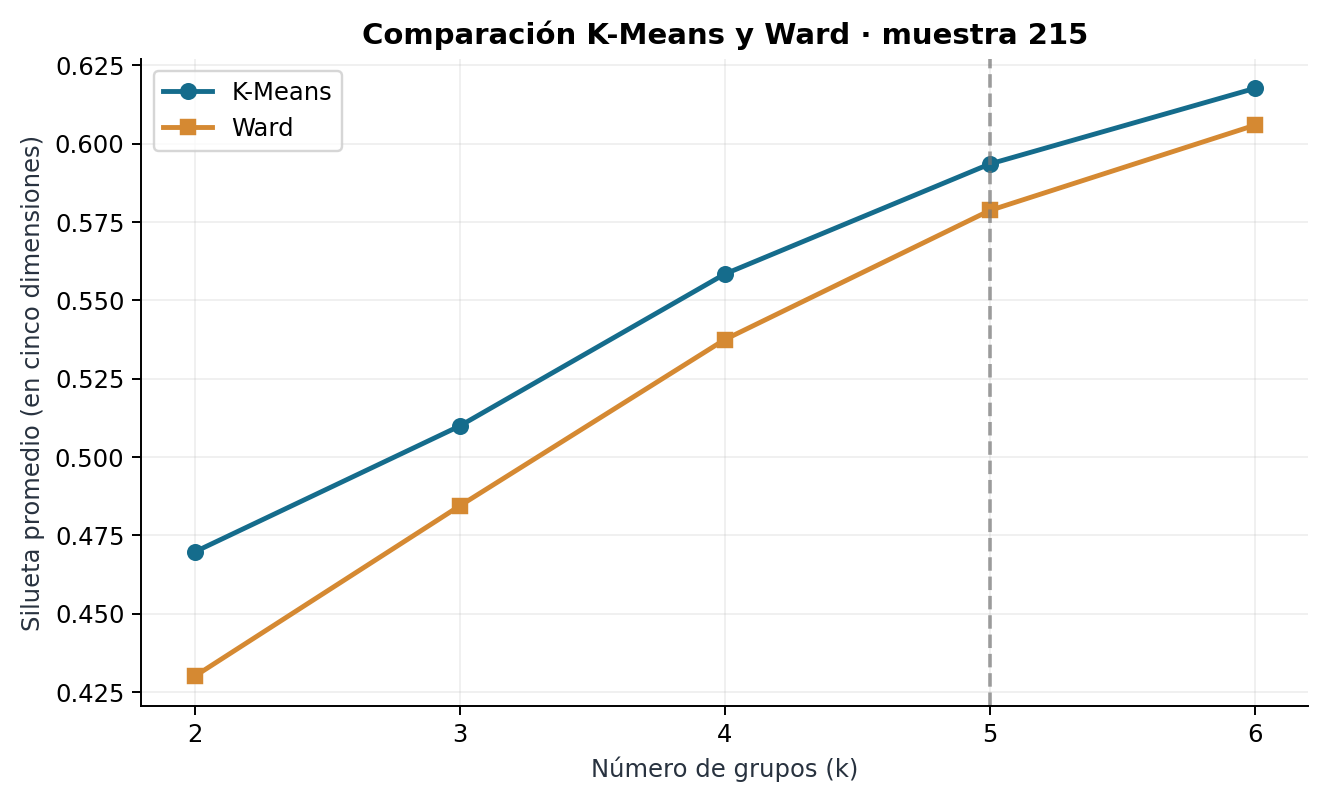
\includegraphics[width=.87\linewidth]{01_comparacion_silueta.png}
\caption{Silueta promedio por número de grupos y algoritmo. Las diferencias de \(k\) no deben resolverse únicamente por el máximo numérico.}\label{fig:silueta}
\end{figure}

Se recomienda \textbf{K-Means, \(k=5\)}, como \emph{propuesta descriptiva provisional}, no como solución única o definitiva: se obtienen cinco patrones de gestión con grupos de 18 a 107 municipios. Para \(k=6\) mejora la silueta, pero aparece un subconjunto de 10 municipios definido por recuperación relativa alta; se documenta en lugar de ocultarlo. Para \(k=4\) los grupos son más compactos, aunque unifican prácticas orgánicas distintas. En \(k=5\) la silueta K-Means fue \(0{,}593507\) y Ward \(0{,}578667\). Las particiones de ambos métodos alcanzan ARI \(0{,}879070\) (el ARI es invariante a los nombres de los grupos \parencite{sklearnARI}).

Las cinco inicializaciones de K-Means, \(k=5\), alcanzaron ARI medio \(0{,}994993\) (mínimo \(0{,}987483\)). En cambio, al excluir los 11 ceros RI ambiguos (215 vs. 204; ARI sobre los \emph{mismos 204 registros}), K-Means \(k=5\) obtuvo \(0{,}841207\), que equivale a 25 cambios de asignación después de alinear etiquetas óptimamente. Ward \(k=5\) obtuvo ARI 1,000 entre escenarios; para K-Means \(k=4\) y \(k=6\), ese ARI también fue 1,000. Se concluye que \(k=5\) es estable frente a semillas, \emph{no perfectamente estable} frente a decisiones de inclusión.

\section{Sensibilidad ante la escala y los valores absolutos}
El tratamiento sin estandarización adicional se respetó como escenario principal del Hito 2. Se ajustó un Z-score con \(n=215\) y se aplicó sin volver a estimar a ambas matrices. Para \(k=5\), K-Means cambió moderadamente (ARI 0,828 frente al original). Sustituir la intensidad relativa RI por RI absoluto transformado produjo ARI 0,685 y añadir \(\log(1+\mathrm{CRR})\) estandarizado como sexta característica redujo el ARI a 0,340. Esto sugiere que la escala operativa puede modificar sustancialmente la partición cuando se usa para calcular distancias. Las medianas de CRR por perfil se reportan de manera \emph{descriptiva}, no causal ni como variable oculta del agrupamiento.

\section{Actividad 7: PCA para visualizar e interpretar}
PCA se ajustó a las mismas cinco variables empleadas para agrupar \parencite{sklearnPCA}. PC1 explica \textbf{46,6633\,\%} de la varianza, PC2 \textbf{18,0605\,\%}; acumulada PC1+PC2: \textbf{64,7238\,\%}. Las contribuciones \((v_{ij}^2\times100)\) más importantes en PC1 son orgánicos (48,16\,\%) y recolección diferenciada (41,47\,\%). PC2 queda dominado por el indicador de botadero (94,60\,\%). El signo de los componentes es convencional y no representa bondad/maldad.

\begin{figure}[htbp]\centering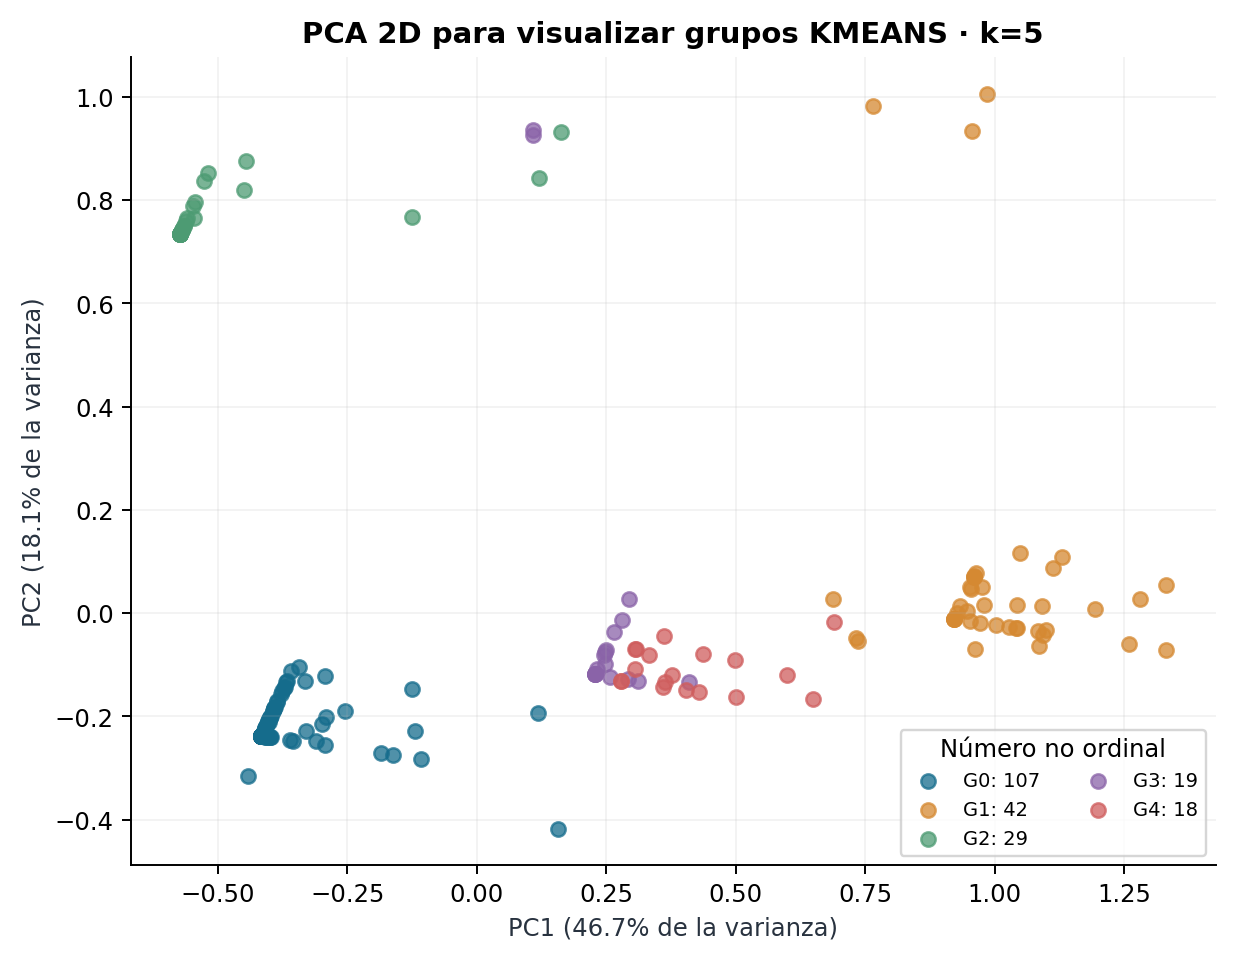
\includegraphics[width=.92\linewidth]{03_pca_kmeans_k5.png}
\caption{Proyección PCA del resultado K-Means \(k=5\). Los colores representan grupos obtenidos antes de PCA; no se calculó la silueta aquí.}\label{fig:pca}
\end{figure}

\section{Actividad 8: perfiles, ejemplos y propuestas por grupo}
Los nombres \emph{describen prácticas reportadas}, no un orden de mérito. Los porcentajes se expresan en unidades de origen, no en la escala logarítmica de las distancias. Las medianas RI de algunos grupos son cero porque existe una concentración de reportes nulos.

\begin{table}[htbp]\centering\scriptsize
\setlength\tabcolsep{3.5pt}
\begin{tabular}{@{}lrrrrrr@{}}\toprule
\textbf{Perfil (ID)}&\textbf{n}&\textbf{Barrido}\,\%&\textbf{Dif.}\,\%&\textbf{Org.}\,\%&\textbf{Bot.}\,\%&\textbf{RI med.}\\
&&&&&&\textbf{kg/mes}\\\midrule
G0 Sin difer. ni orgánicos & 107 & 88,5 & 0,4 & 0,0 & 0,0 & 0\\
G1 Difer. y orgánicos & 42 & 78,0 & 96,8 & 100,0 & 7,1 & 1.020,84\\
G2 Botadero, poca difer. & 29 & 81,4 & 0,5 & 6,9 & 100,0 & 0\\
G3 Difer. sin orgánicos & 19 & 78,6 & 99,9 & 0,0 & 10,5 & 0\\
G4 Orgánicos, poca difer. & 18 & 82,8 & 5,4 & 100,0 & 0,0 & 1.029,38\\\bottomrule
\end{tabular}
\caption{Perfiles provisionales K-Means \(k=5\), 215 municipios. Barrido y diferenciada: medias porcentuales. Orgánico y botadero: proporción de municipios con indicador 1. Recuperación RI: mediana de kilogramos por mes.}\label{tab:perfiles}
\end{table}

\begin{figure}[htbp]\centering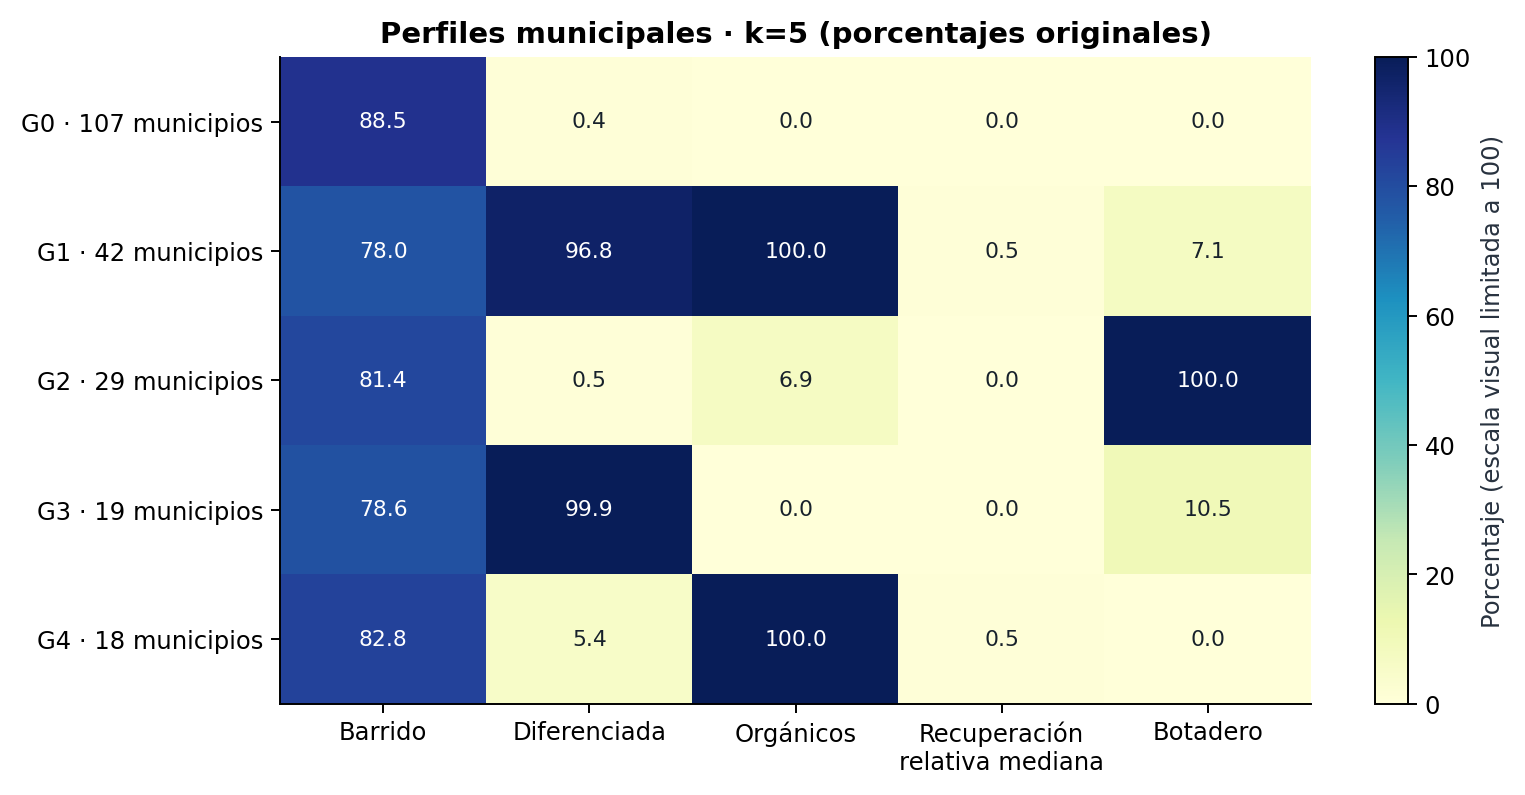
\includegraphics[width=.96\linewidth]{06_perfiles_porcentajes.png}
\caption{Resumen visual de perfiles en porcentajes; el porcentaje de recuperación relativa es mediana. Las variables binarias indican actividad reportada, no rendimiento medido.}\label{fig:perfiles}
\end{figure}

Ejemplos de municipios cercanos al centroide (\emph{no líderes ni modelos}): G0 Jama; G1 Pastaza; G2 Chone; G3 Quito; G4 Cuenca. La identificación exacta y provincias figuran en \texttt{municipios\_representativos\_k5.csv}. Las posibles preguntas de apoyo son:
\begin{itemize}
\item \textbf{G0:} comprobar prácticas reales de separación y viabilidad de pilotos; no inferir ausencia absoluta de toda gestión.
\item \textbf{G1:} comprobar si las actividades de separación y orgánicos reportadas se traducen en recuperación efectiva y sostenida.
\item \textbf{G2:} caracterizar condiciones técnicas y necesidades de información sobre el sitio principal de disposición, antes de proponer cambios.
\item \textbf{G3:} investigar la brecha entre recolección diferenciada declarada y actividad orgánica no reportada; precisar flujos y destinos.
\item \textbf{G4:} explorar si la actividad orgánica se integra operativamente con recolección diferenciada y cómo se registra su cantidad.
\end{itemize}

\section{Limitaciones, precauciones y traspaso al Hito 4}
Se preservaron cuatro coberturas \texttt{CSB>1} y no se eliminaron perfiles numéricos repetidos ni municipios por elevar la silueta. Los 11 ceros ambiguos siguen como cero reportado en el escenario 215 y generan sensibilidad. Los nombres y códigos cantonales proceden de tablas del equipo; ciertos ceros iniciales de \texttt{CantonId} pueden haberse perdido en Excel. No se reconstruyeron claves sin contraste con la base INEC integral. El dato de actividad orgánica no implica volumen procesado; las etiquetas no expresan desempeño municipal.

El producto se limita a \emph{una edición}. Antes de decisiones operativas se necesitan reportes administrativos verificables, información de infraestructura, series temporales y validación local. No se presentan mapas porque no se realizó una correspondencia territorial verificada. La persona a cargo del \textbf{Hito 4} integrará estos resultados y sus límites en el notebook final reproducible y en un \emph{informe divulgativo independiente}, con el formato LaTeX PUCE dispuesto en \textit{formatoInforme.pdf}. Este borrador técnico no sustituye ese informe.

\printbibliography[heading=bibintoc,title={Referencias y fuentes verificables}]
\end{document}
